\documentclass{article}

\usepackage{biblatex}
\addbibresource{biblio.bib}
\usepackage{graphicx}
\usepackage[utf8]{inputenc}
\usepackage[margin=1.2in]{geometry}
\usepackage{color}
\usepackage{amsmath}
\usepackage{hyperref}
\usepackage{listings}
\usepackage{xcolor}

\definecolor{methods_yellow}{rgb}{0.7, 0.6, 0.0}
\definecolor{variable_bleu}{rgb}{0.3, 0.6, 0.8}
\definecolor{keywords_purple}{rgb}{0.7, 0.0, 0.6}
\definecolor{comments_green}{rgb}{0.1, 0.5, 0.1}
\definecolor{listing_background}{rgb}{0.15, 0.15, 0.15}
\definecolor{dark_white}{rgb}{0.9, 0.9, 0.9}

\lstset{
  language=Python,
  keywordstyle=\color{keywords_purple},
  identifierstyle=\color{variable_bleu},
  emph={solve_mesh,compute_element_stiffness_matrix,
        apply_boundary_conditions,compute_rigidity_matrix},
  emphstyle=\color{methods_yellow},
  commentstyle=\color{comments_green},
  backgroundcolor=\color{listing_background},
  basicstyle=\ttfamily\small\color{dark_white},
  xleftmargin=1em,
  framexleftmargin=0.5em,
  framexrightmargin=0.5em,
  frame=single,
  breaklines=true,
  tabsize=2
}

\begin{document}

\begin{titlepage}
    \begin{titlepage}      
        \begin{center}
            
\includegraphics[width=7cm]{img/Logo_IMT_Atlantique.png}
            \\[1.9cm]
            {\LARGE IMT Atlantique}\\[1.5cm]
            
			{\color{black} \rule{\textwidth}{1pt}}

            \linespread{1.2}
            \vspace{0.5cm}
            \huge {\textbf{Électrostatique : modélisation de l'effet de pointe
             par méthode des éléments finis}}
            \vspace{1cm}
            \linespread{1.2}
			{\color{black} \rule{\textwidth}{1pt}}
            \Large {BLOCH Maxime} \\
            \Large {LEHEL Eliaz} \\[1cm]
            \Large {Mars 2025}
            
        \end{center}
    \end{titlepage}
\end{titlepage}

\section*{Introduction}

\hspace{1cm}
Nous nous proposons dans ce travail d'utiliser la méthode des éléments finis
pour modéliser l'effet de pointe dans un champ électrostatique.

\section{Situation physique}

\begin{figure}[!h]
    \centering
    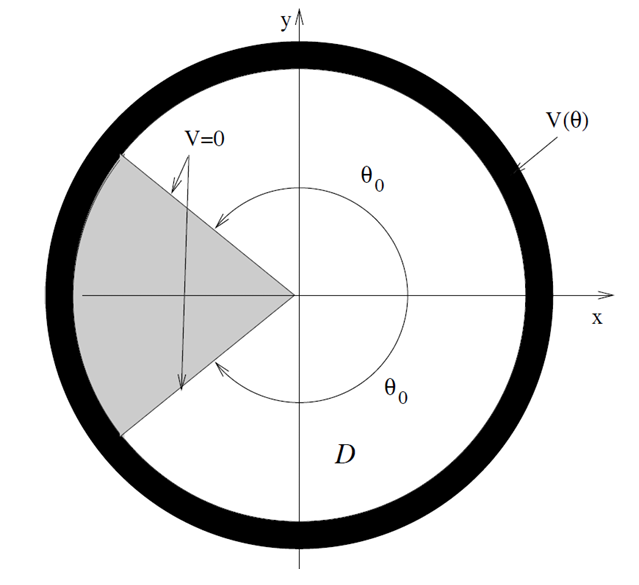
\includegraphics[scale=0.7]{img/schema.png}
    \caption{Modélisation de la pointe}
    \label{fig:pointe}
\end{figure}

\hspace{0.5cm}
La figure \ref{fig:pointe} représente une pointe (en gris) dont les bords sont
maintenus à un potentiel $V=0$ et les contours de la cavité (en noir) à
un potentiel constant $V(\theta)$ non nul.

\begin{equation}
    V(\theta) = 1 - \frac{\theta^2}{\theta_0^2}, \ \text{where } \theta_0=\frac{3\pi}{4}
\end{equation}

Dans ces conditions, le potentiel électrostatique $V$ est solution de l'équation
de Laplace :

\begin{equation}
    \Delta V = 0
\end{equation}

\newpage

\section{Modélisation par éléments finis}

\subsection{Equation à résoudre}

\hspace{0.5cm}
Nous cherchons à résoudre l'équation de Laplace sur un domaine $\Omega$ avec des
conditions aux limites de Dirichlet sur le domaine $\Gamma_D$.

On pose $u$ le potentiel électrostatique. Nous voulons résoudre:

\begin{equation}
   \frac{\partial^2 u}{\partial x^2} + \frac{\partial^2 u}{\partial y^2} = 0
\end{equation}

Nous introduisons les fonctions $v$ sur $\Omega$ le domaine de définition de $u$,
notre potentiel, avec $v \in V = \{H^1(\Omega); v|_{\Gamma_D} = 0 \}$, où
$H^1(\Omega)$ est l'espace de Hilbert des fonctions dérivables au sens des
distributions et carrés intégrables sur $\Omega$.

Pour appliquer la méthode des éléments finis, nous utilisons Green
pour écrire:

\begin{equation}
    \int_\Omega \Delta u(x) v(x) dx = \int_\Omega \nabla u(x) \nabla v(x) dx
    - \int_{\Gamma} \partial_n u(s) v(s) ds
\end{equation}

Par définition, les fonctions tests $v$ sont nulles sur le bord $\Gamma$. Nous avons
donc:

\begin{equation}
    \int_\Omega \nabla u(x) \nabla v(x) dx = 0
    \label{eq:weak_form}
\end{equation}

L'équation \ref{eq:weak_form} est appelée la formulation
faible de notre problème.

Ainsi, nous cherchons $u$ telle que pour tout $v$ dans l'espace
de Hilbert $H^1(\Omega)$, l'équation \ref{eq:weak_form} soit vérifiée.

On peut réécrire cette équation sous la forme suivante:

\begin{equation}
    a(u, v) = 0
\end{equation}

On ajoute maintenant la condition de Dirichlet sur le bord $\Gamma_D$:

\begin{equation}
    u(x) = g(x), \hspace{0.2cm} \forall x \in \Gamma_D
    \Leftrightarrow  u-g \in V
\end{equation}

Dès lors, nous pouvons approcher le problème avec la solution 
$u^h$ dans un espace de dimension finie $V^h$.

On a donc:

\begin{equation}
    a(u^h, v^h) = 0
\end{equation}

On décompose $u^h$ et $v^h$ sur la base des fonctions chapeau
$\{B^h_i\}^{i=N^h}_{i=1}$

\begin{equation}
    u^h = g^h + \sum_{i=1}^{N^h} x_i B^h_i
    \ \text{ et } \ v^h = \sum_{i=1}^{N^h} y_i B^h_i
\end{equation}

Avec $x_i$ les inconnues du problème.

On revient au problème équivalent suivant:

\begin{equation}
    a(u^h - g^h, v^h) = - a(g^h, v^h)
\end{equation}

On pose maintenant les coefficients $A_{ij} = a(B^h_j, B^h_i)$. Ainsi, nous pouvons
réécrire le problème sous forme matricielle:

\begin{equation}
    \sum_{i,j} y_i A_{i,j} x_j
\end{equation}

En posant $g_i = a(g^h, B^h_i)$, ce qui donne $a(g^h, v^h) = \sum_i y_i g_i$,
on obtient le système linéaire suivant:

\begin{equation}
    \sum_{i,j} y_i A_{i,j} x_j = - \sum_i y_i g_i
\end{equation}

Que l'on peut réécrire sous forme matricielle en posant $b$ le vecteur colonne
des $-g_i$ et $x$ le vecteur colonne des $x_i$:

\begin{equation}
    y^T \cdot A \cdot x =  y^T \cdot b
\end{equation}

Ce qui équivaut à résoudre:

\begin{equation}
    A \cdot x = b
\end{equation}

\subsection{Méthode des éléments finis}

Nous devons maintenant assurer le raccord entre les différents éléments.
Pour ce faire, nous considérons dorénavant les fonctions tests
polynomiales $v \in X^h$.

Dès lors, on montre que chaque fonction $v$
est définie par les valeurs qu'elle prend
sur les nœuds du maillage et nous pouvons les écrire comme une combinaison
linéaire des fonctions $B_i$, les fonctions chapeau généralisées.

Ainsi, nous assurons directement la continuité de $v$ sur les éléments en
ayant simplement les mêmes valeurs aux nœuds.

\newpage

\subsection{Maillage du domaine}

\hspace{0.5cm}
Nous allons discrétiser le domaine en éléments finis et résoudre le problème
de Laplace par la méthode des éléments finis. Dans un premier temps,
nous avons choisi de considérer une géométrie simple, mais les calculs
qui vont suivre demeurent généraux jusqu'à la section \ref{sec:cadre_du_pb}.

La figure \ref{fig:pointe_ef} représente la discrétisation du domaine en éléments
finis. Nous nous placerons en deux dimensions.

\begin{figure}[h]
    \centering
    \hspace{1cm} 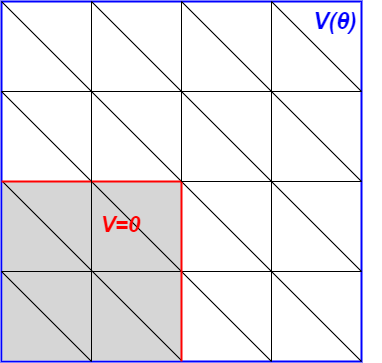
\includegraphics[scale= 0.7]{img/pointe_ef.png}
    \caption{Discretisation du domaine}
    \label{fig:pointe_ef}
\end{figure}

On rappelle qu'on doit résoudre le problème suivant:

\begin{equation}
    \begin{cases}
        u^h \in X^h, \hspace{0.3cm} u^h - g^h \in V^h \\
        a(u^h, v^h) = 0, \hspace{0.3cm} \forall v^h \in V^h
    \end{cases}   
\end{equation}

\newpage

\subsection{Décomposition des polynômes sur un élément}

On réécrit le problème avec des sommes sur chaque élément $[e]$:

\begin{equation}
    a(u^h, v^h) = \sum_{T^{[e]} \in \mathcal{T}^h} \int_{T^{[e]}}
    \sum_{i,j=1}^N a_{ij} \partial_j u ^{[e]} \partial_i v^{[e]} dT^{[e]}
    \label{eq:general_problem}
\end{equation}

Chaque élément $T^{[e]}$ est défini par trois
nœuds (Figure \ref{fig:element}).

\begin{figure}[h]
    \centering
    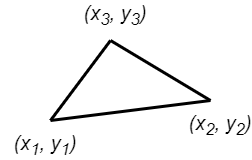
\includegraphics[scale=0.5]{img/element.png}
    \caption{Un élément du maillage}
    \label{fig:element}
\end{figure}

Dans la suite, l'idée sera de décomposer les polynômes
sur chaque élément et de réécrire le problème sous forme
matricielle.

Pour ce faire, on note simplement $u^{[e]}$ et $v^{[e]}$
les fonctions $u$ et $v$ sur l'élément $T^{[e]}$, ainsi que
$u^{[e]}_i$ et $v^{[e]}_i$ les valeurs de $u^{[e]}$ et $v^{[e]}$
au nœud $i$ de l'élément $T^{[e]}$.

\subsection{Matrice de raideur partielle}

On introduit la matrice de raideur partielle
$K^{[e]}$ telle que pour un élément [e]:

\begin{equation}
    \int_{T^{[e]}} \sum_{i,j=1}^2 a_{ij} \partial_j u ^{[e]}
     \partial_i v^{[e]} dT^{[e]} 
     = \left[ v_1^{[e]}, v_2^{[e]},  v_3^{[e]} \right] \cdot K^{[e]}
     \cdot \left[ u_1^{[e]}, u_2^{[e]}, u_3^{[e]} \right]^T
    \label{eq:int_to_K}
\end{equation}

Si nous considérons un seul élément [e], nous pouvons chercher à expliciter
les termes de la matrice de raideur $K^{[e]}$.

On réécrit le problème comme suit:

\begin{equation}
    \left[ v_1^{[e]}, v_2^{[e]},  v_3^{[e]} \right] K^{[e]}
     \left[ u_1^{[e]}, u_2^{[e]}, u_3^{[e]} \right]^T
     = \int_{T^{[e]}} \left[\partial_x v^{[e]},
     \partial_y v^{[e]}\right] A^{[e]} \left[\partial_x u^{[e]},
     \partial_y u^{[e]}\right]^T dT^{[e]}
\end{equation}

Avec $A^{[e]}$ la matrice des coefficients $a_{ij}$.

Nous allons chercher à réécrire ce problème sous forme matricielle
afin d'être capable de calculer les coefficients de $K^{[e]}$.
De cette manière, nous serons capable d'avoir accès au terme
de l'intégrale de l'équation \ref{eq:int_to_K}.

En sélectionnant des polynômes de degré 1 sur un élément $T^{[e]}$,
l'intégrale se réduit à la mesure de l'aire du triangle élémentaire
noté $|T^{[e]}|$ et à moyenner les valeurs de $A^{[e]}$:

\begin{equation}
    \begin{bmatrix}
        v_1^{[e]} & v_2^{[e]} &  v_3^{[e]}
    \end{bmatrix}
    K^{[e]}
    \begin{bmatrix}
        u_1^{[e]} \\ u_2^{[e]} \\ u_3^{[e]}
    \end{bmatrix}
     = |T^{[e]}| \cdot
    \begin{bmatrix}
        \partial_x v^{[e]} & \partial_y v^{[e]}
    \end{bmatrix}
    \overline{A^{[e]}}
    \begin{bmatrix}
        \partial_x u^{[e]} \\ \partial_y u^{[e]}
    \end{bmatrix}
    \label{eq:vKu_eq}
\end{equation}

\subsection{Réécriture sous forme matricielle}

Puisque $u,v \in V^h$, on sait qu'on peut les écrire sous forme
de polynômes de degré 1 en deux dimensions:

\begin{align}
    u^{[e]}(x,y) = \alpha_0^{[e]} + \alpha_1^{[e]} x + \alpha_2^{[e]} y
    = \left[1 \ x \ y\right]
    \left[ \alpha_0^{[e]} \ \alpha_1^{[e]} \ \alpha_2^{[e]} \right]^T \\
    v^{[e]}(x,y) = \beta_0^{[e]} + \beta_1^{[e]} x + \beta_2^{[e]} y
    = \left[1 \ x \ y\right]
    \left[ \beta_0^{[e]} \ \beta_1^{[e]} \ \beta_2^{[e]} \right]^T
\end{align}

Puisqu'on cherche la décomposition de $u$ sur la 
base des fonctions chapeau, on exprime les coefficients de $u$
par rapport à cette base grâce aux sommets de l'élément
sous la forme suivante:

\vspace{0.5cm}

\begin{minipage}{0.45\textwidth}
    \begin{equation*}\begin{cases}
        \alpha_0^{[e]} + \alpha_1^{[e]} x_1
        + \alpha_2^{[e]} y_1 = u^{[e]}_1 \\
        \alpha_0^{[e]} + \alpha_1^{[e]} x_2
        + \alpha_2^{[e]} y_2 = u^{[e]}_2 \\
        \alpha_0^{[e]} + \alpha_1^{[e]} x_3
        + \alpha_2^{[e]} y_3 = u^{[e]}_3
    \end{cases}\end{equation*}
\end{minipage}
\begin{minipage}{0.01\textwidth}
    \centering
    $\Leftrightarrow$
\end{minipage}
\begin{minipage}{0.45\textwidth}
    
    \begin{equation}
        \hspace{-2cm} P^{[e]} \left[\alpha^{[e]}\right] = \left[u^{[e]}\right]
        \label{eq:p_alpha_u}
    \end{equation}
\end{minipage}

\vspace{5mm}

Avec la matrice $P^{[e]}$ définie par:

\begin{equation}
    P^{[e]} = \begin{bmatrix}
        1 & x_1 & y_1 \\
        1 & x_2 & y_2 \\
        1 & x_3 & y_3
    \end{bmatrix}
\end{equation}

Par ailleurs, en dérivant les formes générales
de $u$ et $v$, nous pouvons écrire:

\begin{align}
    \begin{bmatrix}
    \partial_x u^{[e]} \\ \partial_y u^{[e]}
    \end{bmatrix}
    =
    \begin{bmatrix}
    0 & 1 & 0 \\
    0 & 0 & 1
    \end{bmatrix}
    \begin{bmatrix}
    \alpha_0^{[e]} \\ \alpha_1^{[e]} \\ \alpha_2^{[e]}
    \end{bmatrix} \\
    \begin{bmatrix}
    \partial_x v^{[e]} \\ \partial_y v^{[e]}
    \end{bmatrix}
    =
    \begin{bmatrix}
    0 & 1 & 0 \\
    0 & 0 & 1
    \end{bmatrix}
    \begin{bmatrix}
    \beta_0^{[e]} \\ \beta_1^{[e]} \\ \beta_2^{[e]}
    \end{bmatrix}
\end{align}

On pose alors la matrice $D =
\begin{bmatrix}
    0 & 1 & 0 \\
    0 & 0 & 1
\end{bmatrix} $
qui nous permet de dériver simplement les fonctions $u$ et $v$.
On pose les vecteurs suivants:

\begin{equation}
    \begin{bmatrix}
        \partial_x u^{[e]} \\ \partial_y u^{[e]}
    \end{bmatrix}
    =
    \left[ \partial u^{[e]} \right]
    \text{ et }
    \begin{bmatrix}
        \partial_x v^{[e]} \\ \partial_y v^{[e]}
    \end{bmatrix}
    =
    \left[ \partial v^{[e]} \right]
\end{equation}

\begin{equation}
    \begin{bmatrix}
        \beta_0^{[e]} \\ \beta_1^{[e]} \\ \beta_2^{[e]}
    \end{bmatrix}
    = \left[ \beta^{[e]} \right]
    \text{ et }
    \begin{bmatrix}
        \alpha_0^{[e]} \\ \alpha_1^{[e]} \\ \alpha_2^{[e]}
    \end{bmatrix}
    = \left[ \alpha^{[e]} \right]
\end{equation}

\begin{equation}
    \begin{bmatrix}
        u_1^{[e]} \\ u_2^{[e]} \\ u_3^{[e]}
    \end{bmatrix}
    = \left[ u^{[e]} \right]
    \text{ et }
    \begin{bmatrix}
        v_1^{[e]} \\ v_2^{[e]} \\ v_3^{[e]}
    \end{bmatrix}
    = \left[ v^{[e]} \right]
\end{equation}

Avec ces nouvelles matrices, muni de l'équation
\ref{eq:p_alpha_u} et de l'équation \ref{eq:vKu_eq} que l'on réécrit
comme suit:

\begin{equation}
    \left[ v^{[e]} \right]^T K^{[e]} \left[ u^{[e]} \right]
    =
    |T^{[e]}| \left[ \partial v^{[e]} \right]
    \overline{A^{[e]}} \left[ \partial u^{[e]} \right]
\end{equation}

On peut alors réécrire le problème sous forme matricielle:

\vspace{0.4cm}

\begin{equation}
    \left[ v \right]^T K^{[e]} \left[ u \right]
    =
    |T^{[e]}| \left[ \partial v \right]^T \overline{A^{[e]}}
    \left[ \partial u \right]
\end{equation}

\vspace{-0.3cm}

\begin{center} $\Leftrightarrow$ \end{center}

\vspace{-0.6cm}

\begin{equation}
    \left(P^{[e]}\left[\beta^{[e]}\right] \right)^T K^{[e]}
    P^{[e]}\left[\alpha^{[e]}\right] = |T^{[e]}|
    \left(D\left[\beta^{[e]}\right]\right)^T
    \overline{A^{[e]}} D\left[\alpha^{[e]}\right]
\end{equation}

\vspace{0.4cm}

En passant les termes à droite, en simplifiant les
matrices $\left[\alpha\right]$ et $\left[\beta\right]$ par
la droite et la gauche, et en écrivant
$H^{[e]} = \left( P^{[e]}\right)^{-1}$, on obtient:

\begin{equation}
    K^{[e]} = \left(H^{[e]}\right)^T D^T
    \left( |T| \overline{A^{[e]}} \right) D H^{[e]}
\end{equation}

Notez qu'ici, $D$ est de taille 2x3, $\overline{A^{[e]}}$
de taille 2x2 et $H^{[e]}$ de taille 3x3.

\subsection{Expression des matrices dans le cadre du problème}
\label{sec:cadre_du_pb}

En pratique, avec notre problème, nous savons que:

\begin{equation}
    \overline{A^{[e]}} =
    \begin{bmatrix}
        1 & 0 \\ 0 & 1
    \end{bmatrix}
\end{equation}

Car, rappelons-le, notre formulation faible d'origine est

\begin{equation}
    \int_\Omega \nabla u(x) \nabla v(x) dx = 0
\end{equation}

Nous avons maintenant besoin de connaître la matrice $H^{[e]}$
et la valeur de $|T|$.

Notons $h$ la longueur d'un côté de l'élément [e]. Nous avons donc
$h = x_2 - x_1 = y_2 - y_1$. Dès lors,

\begin{equation}
    |T| = \frac{1}{2} h^2
\end{equation}


Par ailleurs, nous pouvons inverser la matrice $P^{[e]}$ pour obtenir
la matrice $H^{[e]}$. Par calcul, on trouve:

\begin{equation}
    H^{[e]} = \frac{1}{h^2}
    \begin{bmatrix}
        x_2 y_2 - x_1 y_1 & -hx_1 & -hy_1 \\
        -h & h & 0 \\
        -h & 0 & h
    \end{bmatrix}
\end{equation}

Ces simplifications pourraient être faites dans notre code pour
accélérer les calculs, mais en pratique, on constate que le temps de
calcul est principalement occupé par la reconstruction des valeurs
en chaque point du plan (x, y) (pour une certaine résolution donnée)
plutôt que par la résolution elle-même.

Nous avons donc choisi de garder dans notre solveur une forme générale
du problème telle que présentée à la section précédente.
(La forme de la matrice $A^{[e]}$ est cependant conservée égale à l'identité,
car cette matrice dépend du problème physique et non de la géométrie.)

Ceci nous permet, comme nous le verrons dans la suite,
d'adopter au besoin de nouvelles géométries.

\subsection{Assemblage}

Maintenant dotés des matrices de rigité élémentaires $K^{[e]}$
sur chaque élément, l'équation \ref{eq:general_problem} nous permet
de connaitre les coefficients de $K$, la matrice de rigidité globale
du problème.

En effet, nous avons la correspondance suivante:

\begin{equation}
    \begin{bmatrix}
        v^h_1 & \cdots & v^h_N
    \end{bmatrix}
    K
    \begin{bmatrix}
        u^h_1 \\ \vdots \\ u^h_N
    \end{bmatrix}
    = \sum_{T^{[e]} \in \mathcal{T}^h}
    \begin{bmatrix}
        v^{[e]}_1 & v^{[e]}_2 & v^{[e]}_3
    \end{bmatrix}
    K^{[e]}
    \begin{bmatrix}
        u^{[e]}_1 \\ u^{[e]}_2 \\ u^{[e]}_3
    \end{bmatrix}
    \label{eq:assemblage}
\end{equation}

Ce que nous dit cette équation, c'est que pour chaque nœud,
la valeur de K est la somme de toutes les valeurs de $K^{[e]}$
correspondantes à ce nœud. En effet, chaque élément [e] est
défini par trois nœuds, et chaque nœud est partagé par trois
éléments, donc une matrice $K^{[e]}$ contient
plusieurs fois les contributions de chaque nœud.

\subsection{Conditions limites}

Il ne reste plus qu'à définir les conditions limites de notre système.

Si aucune contrainte n'existait, le système à résoudre serait:

\begin{equation}
    K \left[u^h\right]^T = \left[0\right]
\end{equation}

Mais certaines contributions doivent être retirées de la matrice K.
En effet, il ne faut pas calculer les variations du nœud $i$ lorsque
celui-ci est sur le bord, donc les contributions des autres nœud
à la valeur en $i$ doivent être éliminées. Pour ce faire, il suffit
de fixer à $0$ la colonne $i$ de la matrice $K$
(sauf la valeur en $(i, i)$, ainsi le nœud $i$ sera le seul à contribuer
à sa propre valeur, et on élimine la variation) et définir une valeur
fixe dans le second membre à la place de $0$.

Admettons dans l'exemple suivant que le nœud $i$ se trouve au bord et
est fixée à la valeur $U_i$
Voici les modifications à apporter à la matrice:

\begin{equation}
    \begin{bmatrix}
        K_{1,1} & \cdots & K_{i,1} = 0 & \cdots & K_{1,N} \\
        \vdots & \ddots & \vdots & \ddots & \vdots \\
        \vdots & \ddots & K_{i,i} = 1 & \ddots & \vdots \\
        \vdots & \ddots & \vdots & \ddots & \vdots \\
        K_{N,1} & \cdots & K_{i,N}=0 & \cdots & K_{N,N}
    \end{bmatrix}
    \begin{bmatrix}
        u^h_1 \\ \vdots \\ u^h_N
    \end{bmatrix}
    =
    \begin{bmatrix}
        0 \\ \vdots \\ U_i \\ \vdots \\ 0
    \end{bmatrix}
\end{equation}

En notant le membre de droite $F$ et $K^*$ la nouvelle
matrice de rigidité prenant en compte les conditions aux limites,
il en découle simplement un système linéaire à résoudre:

\begin{equation}
    K^*
    \begin{bmatrix}
        u^h_1 \\ \vdots \\ u^h_N
    \end{bmatrix}
    = F
\end{equation}

Et c'est bien ce calcul qui sera réalisé dans notre code.

\newpage

\section{Présentation du code}

L'architecture du code, la présentation des classes et de leurs
méthodes est déjà décrites extensivement dans le \verb|README|
du projet ainsi que sur le wiki associée.
(\href{https://github.com/LuciferC-137/FiniteElementElec}{Lien vers GitHub})

Dans cette section est donc détaillé le fonctionnement
mathématique du solveur et comment il implémente les équations
présentées précédemment.

Il y a quatre méthodes principales dans le solveur:

\begin{itemize}
    \item \verb|solve_mesh()|
    \item \verb|compute_rigidity_matrix()|
    \item \verb|apply_boundary_conditions()|
    \item \verb|compute_element_stiffness_matrix()|
\end{itemize}

La première résout le problème en appelant les autres.
La deuxième calcule la matrice de raideur $K$ nécessaire à la
résolution du problème, la troisième applique les conditions
limites à la matrice de raideur pour obtenir $K^*$ et $F$, et la dernière calcule
une matrice élémentaire $K^{[e]}$.

Bien évidemment, elles ne sont pas appelées dans cet ordre. Voici
comment se déroule l'algorithme:

\begin{enumerate}
    \item Pour chaque éléments du maillage,
    on calcule la matrice de raideur élémentaire $K^{[e]}$.
    \item Pour chaque noeud, on ajoute ses contributions en "ajoutant" $K^{[e]}$ à l'endroit approprié de $K$.
    \item On applique les conditions limites à $K$ pour obtenir $K^*$ et on détermine $F$.
    \item On résout le système linéaire $K^* \cdot u = F$.
\end{enumerate}

Une version de pseudo-code simplifiée et verbalisée de chaque méthode 
est présentée au listing \ref{lst:solver} ci-après.

\newpage

\begin{lstlisting}[caption={Structure simplifiée du solveur} \label{lst:solver}]
    def solve_mesh():
        # On cree la matrice avec toutes les contributions
        K = compute_rigidity_matrix()
        F = np.zeros(mesh.size())
        # On s'assure de retirer les contributions des noeuds a valeur fixe
        apply_boundary_conditions(K, F, mesh)
        # On appel numpy pour resoudre le systeme lineaire
        u = np.linalg.solve(K, F)
        return u
    
    def compute_rigidity_matrix():
        K = np.zeros((n_nodes, n_nodes))
        for element in mesh.elements():
            # Pour chaque element, on rempli Ke
            Ke = compute_element_stiffness_matrix(element)
            for i, node_i in element.nodes:
                for j, node_j in element.nodes:
                    # On ajoute le coeff de Ke correspondant a la
                    # contribution entre deux noeuds a la matrice K
                    K[node_i.index, node_j.index] += Ke[i, j]
        return K
    
    def compute_element_stiffness_matrix(element):
        x = [node.x for node in element]
        y = [node.y for node in element]

        Pe = np.array([[1, x[0], y[0]],
                       [1, x[1], y[1]],
                       [1, x[2], y[2]]])
        Ae = np.array([[1, 0], [0, 1]])
        He = np.linalg.inv(Pe) # Inversement de la matrice Pe
        Te = 0.5 * np.abs(np.linalg.det(Pe)) # Calcul de l'aire du triangle
        D = np.array([[0, 1, 0],
                      [0, 0, 1]]) # Matrice de derivation
        DT = np.array([[0, 0],
                       [1, 0],
                       [0, 1]]) # Transpose de D

        Ke = np.transpose(He) @ DT @ Ae @ D @ He * Te # Solution elementaire
        return Ke

    def apply_boundary_conditions(K):
        for i in range(mesh.size()):
            if mesh[i].value is not None:
                # Si on a une condition limite au noeud i
                K[i, :] = 0
                # Alors on retire toutes les contributions des autres noeuds
                K[i, i] = 1
                # On devient le seul noeud a participer a notre valeur
                F[i] = mesh[i].value
                # Et la solution pour ce noeud sera nous-meme
    
    \end{lstlisting}

\newpage

\section{Comparaison des résultats avec la théorie}




\end{document}